\section{Existing work}

As I am now three years into my PhD, my research builds on significant prior work. First and foremost, my CORGIS project has already been used in several introductory programming experiences, and seen publication at multiple venues, including two very successful workshops.
My more recent work with Kennel represents a largely unpublished effort, but its key elements have already seen successful deployment in the Computational Thinking class.

\subsection{CORGIS}

My primary research project for the first two years of my dissertation led to CORGIS: Collections of Real-time, Giant, Interesting, Situated Datasets.
This project's goal is to make simplistic data sources available to learners early in their programming experience, so that they can explore Big Data Science contexts.

\subsubsection{Technical Infrastructure}

The foundation of this proposal rests on prior work developing the RealTimeWeb project, a software architecture framework that provides introductory programming students with an easy way to access and manipulate distributed real-time data\cite{bart-transforming}.
Real-time data is a specific branch of Big Data -- specifically, high velocity data.

As our focus shifts from real-time data to big data in general, we have renamed our overarching project from RealTimeWeb to CORGIS. Our work is now available at \url{http://think.cs.vt.edu/corgis/}. As a successor to the RealTimeWeb project, CORGIS retains all the previously developed libraries for accessing high velocity data; however, it also contains our new libraries for working with high volume data.
These libraries are paired with potential assignments and helpful documentation for deployment.
Long term, we intend to gather and disseminate data on the success of these libraries, with the hopes to establish a community of developers and educators that create new resources.
For clarity's sake, we use the name RealTimeWeb to refer to the architecture we have developed to rapidly connect to high velocity data streams.

At the heart of our project are carefully engineered, open-source client libraries through which students can access the data provided by real-time web services.
We provide client libraries for a number of data sources, such as business reviews from Yelp, weather forecasts from the National Weather Service, and social content from link-sharing site Reddit.com.
Each of these client libraries is in turn available for three common beginner languages: Java, Python, and Racket. 
These libraries do more than just streamline the process of accessing distributed data, however; each library is built with a persistence layer that enables the library to work without an internet connection.
Not only does this ensure that students without a solid internet connection can maintain productivity, it also simplifies developing unit tests. 
In fact, this technical scaffolding for the students circumvents most of the difficulties of distributed computing, including HTTP access, data validation, and result parsing.
Figure \ref{fig-cla} demonstrates the architecture used in our libraries.

The persistence layer is implemented using a caching mechanism, but not a traditional one.
In a conventional caching system, the result of every call made to the external service is memoized using a key-value store, often with a timestamp in order to expire out-of-date data.
In our caching system, an instructor preloads the cache with a sequence of data values for each expected call to the external service.
Although this limits the number of possible calls to the external service, it improves the consistency of the experience.
Instructors can specify policies for how the system returns data -- if the cache runs out, it could restart with the initial result, a developer-specified ``empty'' result, or repeatedly return the final result.
For example, consider the United States Geological Services' Earthquake data stream, which exposes a function to retrieve a list of earthquakes around the world for a given time period (e.g., past hour, past day, past week, etc.). 
The instructor could provide a cache to simulate a period of high seismic activity, returning a large number of earthquakes every time the function is called.
If the user exhausts the data in the cache, it might be programmed to return an empty list, signaling no further activity.

\begin{wrapfigure}{R}{0.5\textwidth}
    \begin{center}
			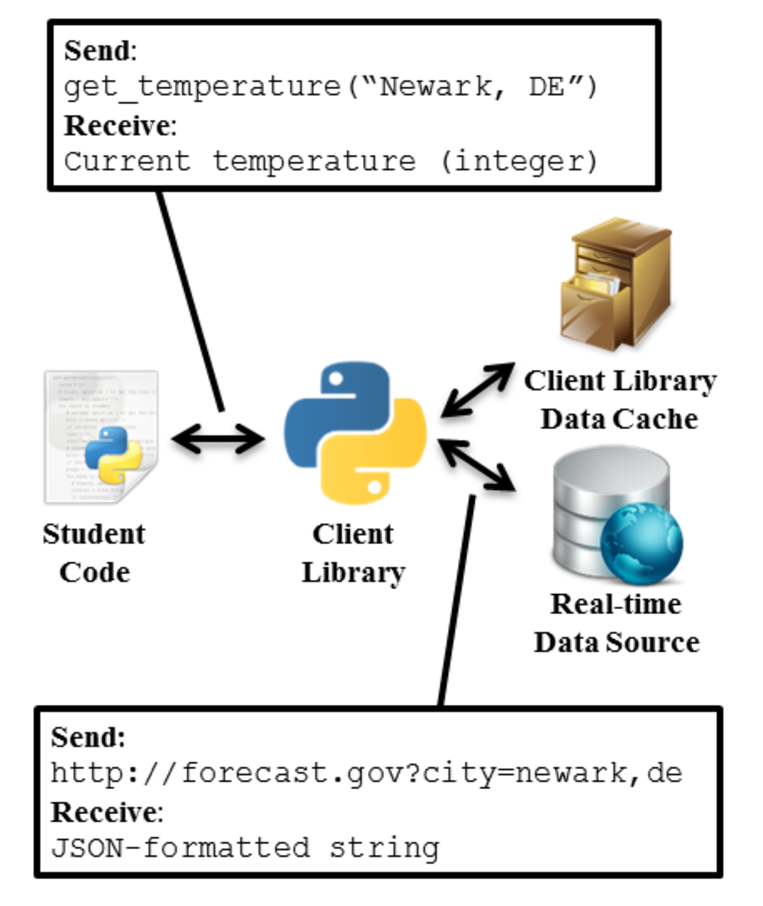
\psfig{file=images/rtw-client-library.eps, width=\linewidth}
			%\includegraphics[width=0.48\textwidth]{"images/rtw-client-library"}
    \end{center}
    \vspace{-\bigskipamount}
    \caption{RealTimeWeb Client Library Architecture}
    \label{fig-cla}
\end{wrapfigure}

Our High Volume libraries often work by providing sampled versions of the data internally, so that students can work with faster, representative subsets.
Then, when they are ready for full deployment, they can switch to a ``full production'' mode -- trading speed for quality. 
Most of the work in developing these libraries is organizing the sampled data to load into memory and get processed as quickly and naturally as possible.

An alternative scheme for distributed High Volume libraries uses a more traditional caching strategy -- assuming that the data source is largely static, requests are cached locally.
This caching is typically done using a simple key-value store on the local filesystem.
Limits can be set on the size or lifespan of the data in the cache, allowing the system to update itself according to the velocity of the external data service.
Using open-source REST API generating tools such as Eve~\cite{Eve}, existing high volume datasets can be quickly transformed into distributed datasets, alleviating the issues of data storage and transmission.

\subsubsection{Semi-Automatic Library Generation}

Our client libraries are easily available through a curated, online gallery; each library is designed to be quickly adapted to instructors' specific academic desires. 
This gallery also provides a tool for rapidly prototyping new libraries based on our framework.
As an open-source project, we encourage collaborators to explore and extend the tools that we have created.

The process of connecting to online data sources is fairly uniform: performing an HTTP request to a URL returns formatted data (typically JSON or XML). 
This information must then be parsed into native data structures, and then filtered and transformed into an appropriate domain object using the language's proper construct (e.g., structs for Racket, classes for Java).
We've established a JSON-based client library specification file format that can be compiled to appropriate source code in each of the three target languages using the modern templating language Jinja2. 
This compiler can be easily extended to new languages by providing a template.
This specification format has two major components: the functions, which connect to the relevant URL endpoints, and the domain objects, that are generated from a successful HTTP request. 
This open-source tool has been used to successfully and rapidly develop a number of the existing client libraries.

\subsubsection{Contextualizing with CORGIS}

The RealTimeWeb toolchain has been deployed for several semesters in introductory Computer Science courses for majors, ranging from the first course all the way to a Data Structures level course.
These integrations ranged from small assignments to entire semester projects using the software.
So far, the focus of the evaluation has been on the motivational influence of the system.
Quantitative data was collected by surveying students attitudes using well-established motivational frameworks and instruments, and indicates that students tended to find real-time data engaging~\cite{realtimeweb}.
In some courses, qualitative data was gathered through small group interviews, where students attribute increased engagement with the authentic, real-world connection offered by real-time data.
Similar results have been found from its integration in the Computational Thinking course -- students cite working with the realistic data as a key factor in engaging with course materials.

\begin{wrapfigure}{R}{0.5\textwidth}
		\begin{center}
				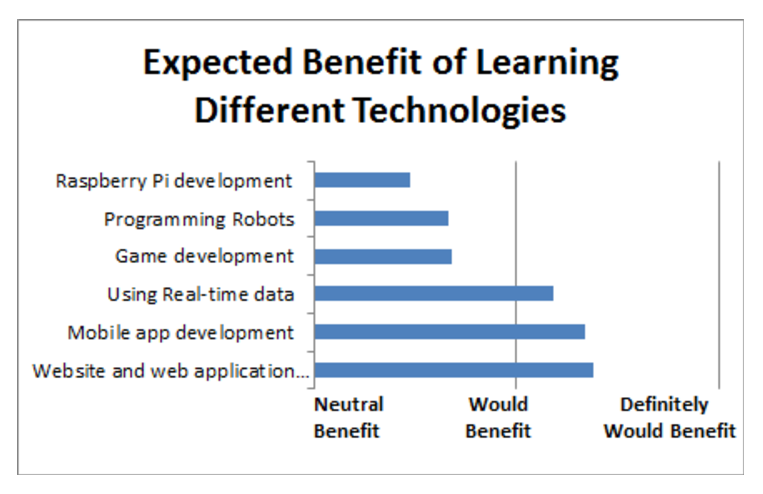
\psfig{file=images/expected-benefit.eps, width=\linewidth}
		\end{center}
		\caption{Students' Perceptions of the Benefit of Working with Learning Different Technologies}
		\label{fig-expected-benefit}
\end{wrapfigure}

\subsubsection{Limitations of CORGIS}

Although CORGIS has more or less successfully solved the problem of integrating high velocity data, and has started supporting high volume data, further work is required to solve the high variety data problem.
Furthermore, there is no principled strategy for pedagogically integrating these tools into a classroom -- instructors tend to choose data streams based on their own situational interest, rather than through a deep understanding of the affordances and limitations of the dataset.
Further work is required both on the technical and philosophical side in order to support these processes.

\subsection{Kennel}

In this section of the paper, I introduce my new online programming environment named Kennel.
The goal of Kennel is to be a beginner-friendly programming environment that scaffolds the learner into a more mature environment while supporting a number of theory-driven, pedagogical objectives.
Internally, Kennel uses a modified version of the open-source Blockly library to provide a block editor, a modified version of the open-source Skulpt library to execute python code, and an unmodified version of the open-source CodeMirror library to provide a text editor.
The system promotes the learning transfer process by supporting Mutual Language Transformation between Blockly and Python -- at any time, code can be transferred back-and-forth between the block editor and the text editor.
This transfer is highly optimized so that there is no usability delay in observing the differences between blocks and text.
Additionally, Python expressions and code blocks can be inlined inside of the Blockly program in order to provide more piece-meal integrations.

The Skulpt execution environment resides entirely within the users' browser, so there is no reliance on an external server to compile and run students' code.
This system also includes a built-in, client-side Property Explorer to support program and data visualization.
This execution environment supports a large number of native Python libraries, including custom ones developed for Big Data analysis.
The long-term goal of this project is to support a useful set of rich libraries so that sophisticated applications can be developed -- going beyond traditional console-based problems.
In this sense, the project is similar to other Skulpt-based environments such as Pythy and CodeSkulptor.
However, Kennel seeks to maintain 100\% compatibility with existing Python APIs so that all code written is authentic.

\begin{wrapfigure}{R}{0.5\textwidth}
\label{fig-blockly-custom}
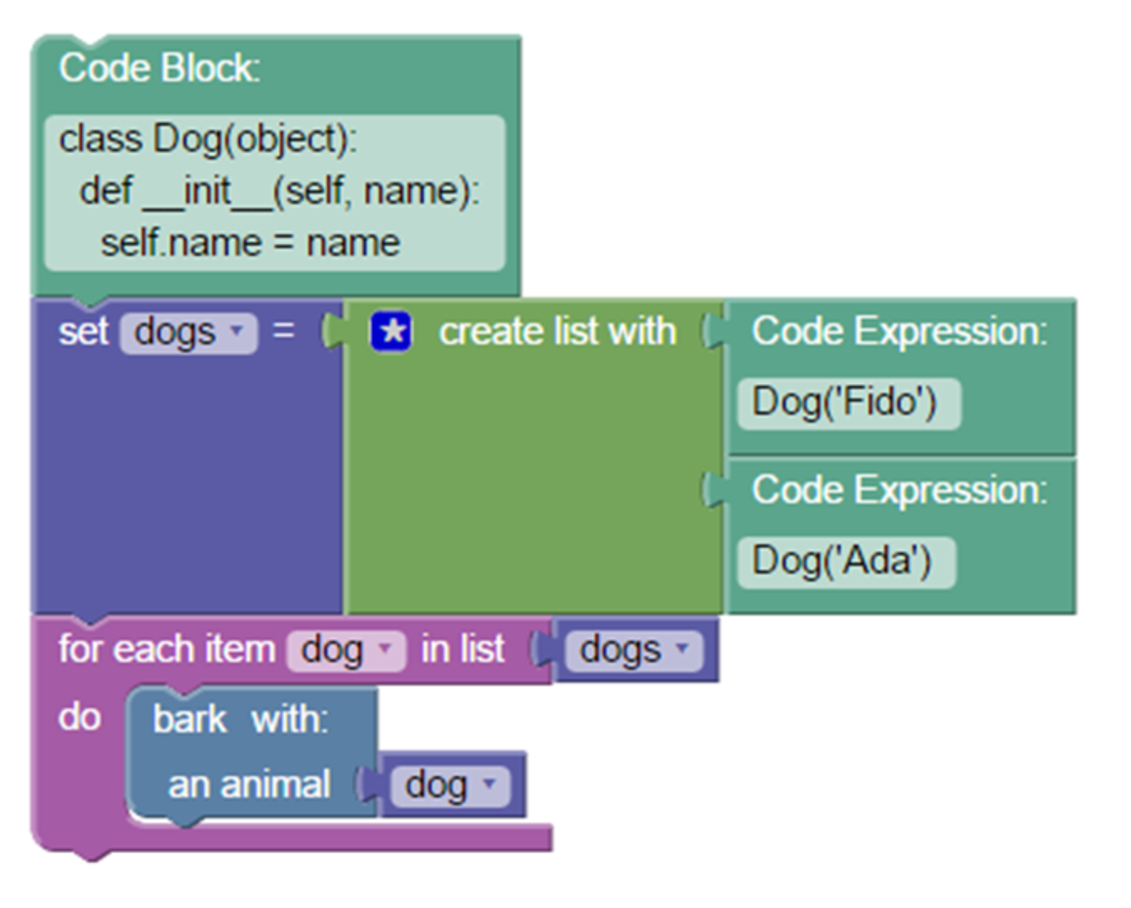
\psfig{file=images/blockly-custom.eps, width=\linewidth}
\caption{Code Block, Code Expression, and user-defined Function blocks can be used to write inline Python code}
\end{wrapfigure}

Kennel is not just a code-authoring environment but also a system for guided practice.
Instructors can create problems with interactive feedback.
As students complete and struggle with milestones within the problem, they can be given just-in-time feedback, support, and encouragement.
As they complete problems, this data can be reported to an interested central location, suitable for grading and course completion information.
The system also tracks a number of events and user interactions for fine-grained analysis.

\subsubsection{Mutual Language Translation}

Work by Weintrop on the transition from Snap to Python offers a number of ways to mediate the transfer through programming tools. 
One of the largest findings is that being able to write inline code inside a Block-based language is extremely helpful to students' learning \cite{Weintrop}.
Figure \ref{fig-blockly-custom} demonstrates how Blockly can support arbitrary code execution through the Code Block, Code Expression, and user-defined Function blocks.
This idea can be pushed further to allow students to convert their block code to textual form and then translate the textual form back to blocks.
This approach, Mutual Language Translation, is also being explored by Matsuzawa\cite{Matsuzawa} to support the transition from a desktop, block-based programming language to Java in an introductory programming class. 
Although our core approaches are similar, there are major differences.
First, translating a dynamically-typed language is a non-trivial improvement over translating a statically-typed language -- in fact, the former is technically impossible to do with 100\% accuracy, and requires a number of novel solutions in order to achieve a reasonable measure of success.
Second, my version is browser-based version, rather than relying on client-side tools, greatly enhancing the portability and providing more sophisticated student tracking.

Figure \ref{fig-mlt-overview} gives an overview of the flow of code in the environment, and figures \ref{fig-example-blockly} and \ref{fig-example-python} demonstrate the near-equivalency of the output of the two code editors.
Blockly outputs valid python source code, which can be passed into Skulpt in order to retrieve a JSON representation of the Abstract Syntax Tree.
Alternatively, the Python source of the Skulpt program can be edited directly by the user. 
Either way, this AST is parsed using our Py2Block library in order to generate an XML representation that Blockly can transform into its blocks.

Blockly already supports compilation of its blocks to Python, JavaScript, and Dart.
However, this multiple language support comes at a cost of reduced isomorphism - each language has different syntax for their common operations, and it is impossible to create a fully-featured block language with a one-to-one mapping between them.
For example, JavaScript has no support for parallel assignment, a commonly-used feature in Python, while Python does not have increment or decrement operators.

Instead of trying to satisfy multiple languages, we have dropped support for JavaScript in favor of a more full-featured mapping to Python.
Most of the changes are minor details that introduce pythonic syntax details: functions blocks are labeled ``define'', assignment blocks have an ``='' operator, the ``add item to list'' block is renamed to ``append''.
New language features are now also available -- Blockly has been extended to include support for creating and retrieving dictionaries, a crucial data structure in Python.
Some behavior of Blockly has been modified: for instance, the original code creation uses the \texttt{global} keyword within closures in order to prevent beginners from having unexpected behavior with aliased global properties -- however, this introduces additional complexity and may not be useful in a introductory context, where beginners should encounter useful struggles when they attempt to reuse global variables in a local scope.

\subsubsection{Big Data Science}

\begin{wrapfigure}{R}{0.5\textwidth}
\label{fig-mlt-overview}
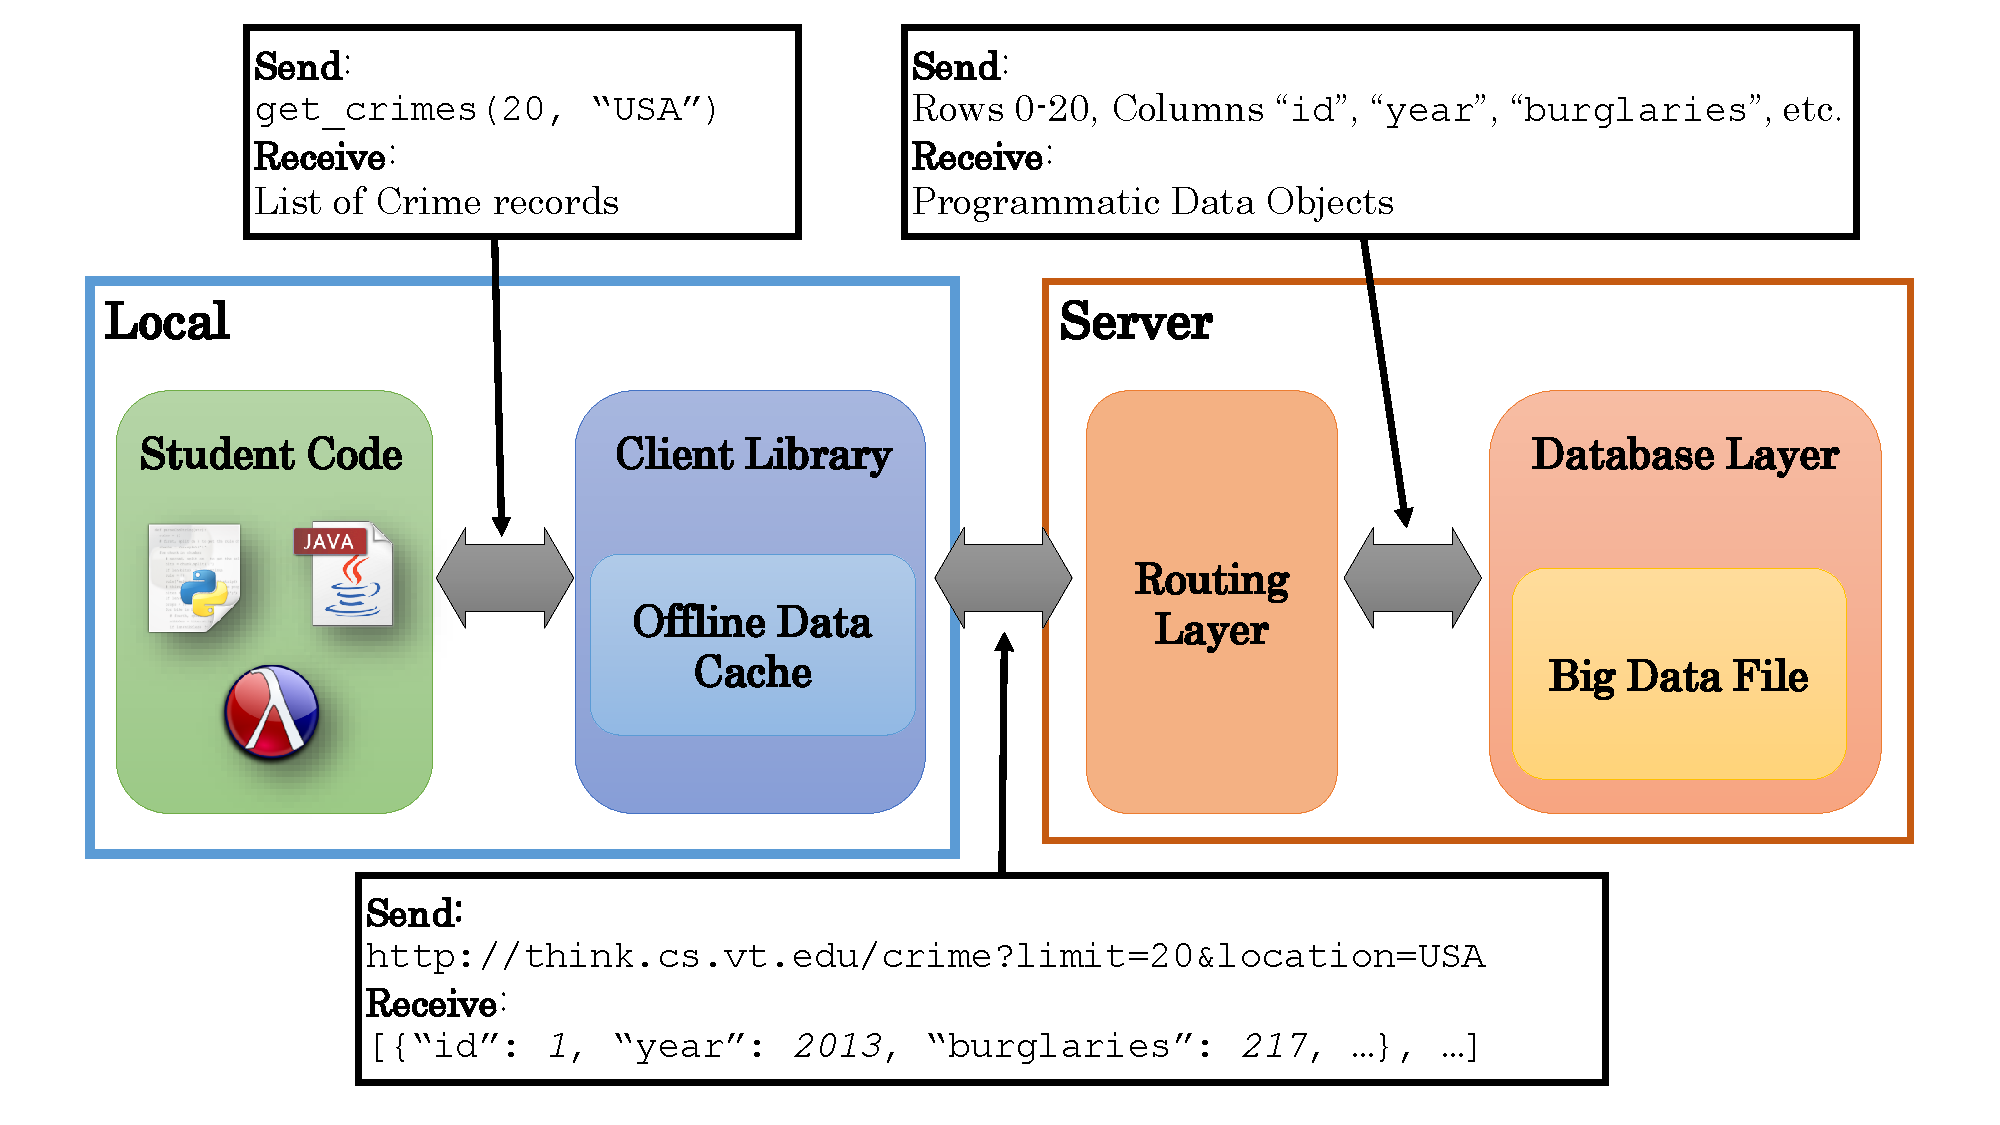
\psfig{file=images/graphics.ps, width=\linewidth}
\caption{The flow of code in the Mutual Language Translation system}
\end{wrapfigure}

In accordance with our motivational theory, we seek to move past interest-based programming into broadly useful programming contexts.
To that end, we use Data Science as an authentic context for teaching introductory computing.
As previously mentioned, Skulpt supports a number of Python APIs, and it can also be extended with any existing pure-python libraries or JavaScript libraries that use the Skulpt API.
We use a fork of Skulpt with partially equivalent implementations for the popular MatPlotlib library~\cite{SkulptMatPlotLib} and also extended it with our own implementation of the CORGIS project.
The Waywaard MatPlotLib API provides a ``plot(list)'' function to create simple line plots.
By basing everything around the MatPlotLib API, students can seamlessly shift to a serious programming environment without loss of code or productivity. 

The CORGIS (Collection of Real-time, Giant, Interesting Datasets) project strives to make it trivial to bring Big Data into introductory programming courses through carefully scaffolded libraries -- including rapidly changing high velocity data (e.g., weather, stocks) or massive high volume datasets (e.g., census and crime report data).
These libraries are pure python, and are rapidly integrated into Skulpt and exposed through the block editor, as seen in figure \ref{fig-example-blockly}.
Data returned from their interface is extremely simple -- usually either primitive (numbers and text) or simply structured (heterogenous dictionaries and homogenous lists), ensuring that students can begin working with Big Data blocks at the earliest possible point in the course.

During the course, students take advantage of the internal caching mechanism of the CORGIS libraries to work on recorded data.
This simplifies the debugging process since programs perform predictably and are no longer dependent on external data services.
When students are ready to run their programs against live data, they can move offline to a traditional programming environment and run in regular production.
This caching mechanism also benefits from an assessment view - a students program can be checked for robustness by invisibly changing the values returned by the big data functions.

\begin{figure*}[ht]
\centering
\begin{minipage}[b]{.75\linewidth}
\caption{Blockly Code}
\label{fig-example-blockly}
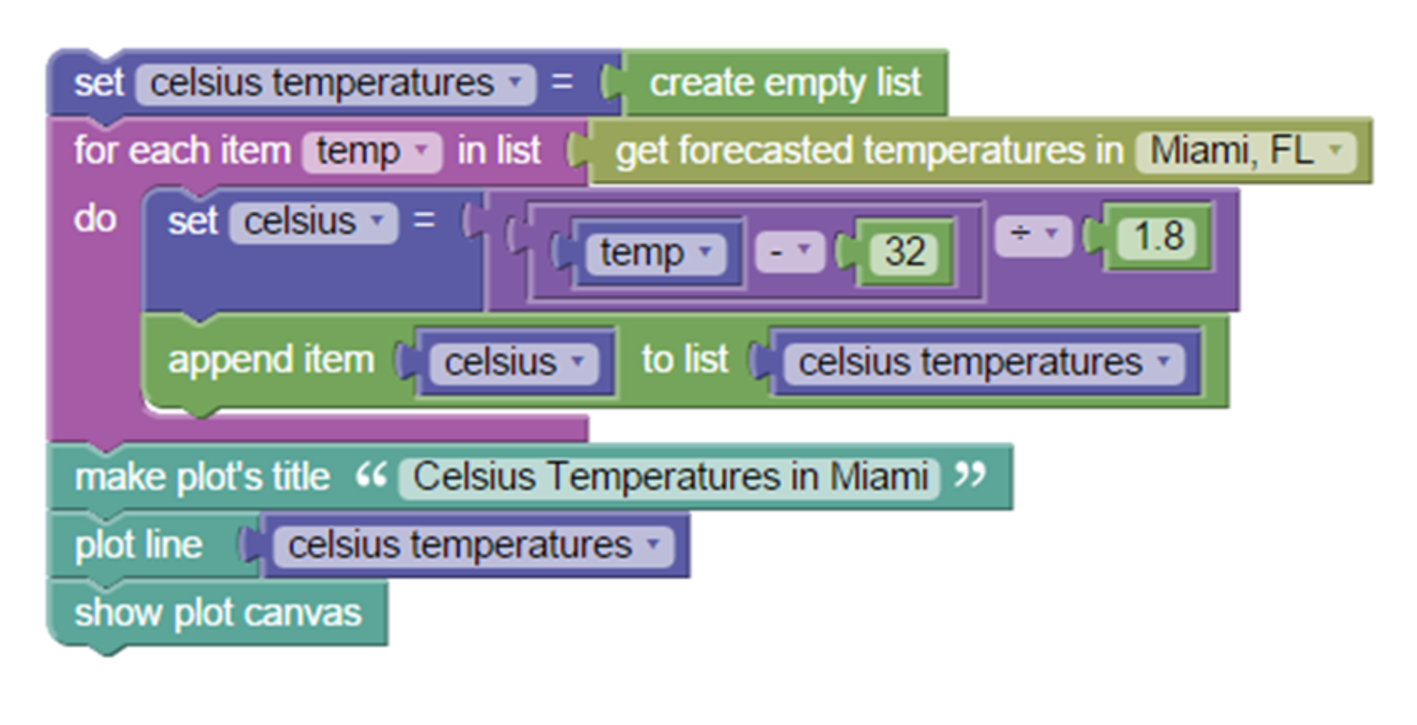
\psfig{file=images/blockly-example.eps, width=\linewidth}
\end{minipage}

\smallskip

\begin{minipage}[b]{.75\linewidth}
\caption{Python Code}
\label{fig-example-python}
\begin{python}
import weather
import matplotlib.pyplot as plt

celsius_temperatures = []
for t in weather.get_temperatures("Miami, FL"):
	celsius = (t - 32) / 1.8
	celsius_temperatures.append(celsius)
plt.title("Celsius Temperatures in Miami")
plt.plot(celsius_temperatures)
plt.show()
\end{python}
\end{minipage}
\end{figure*}


Eventually, more sophisticated visualizations will be required.
Users are often highly motivated to create user interfaces to control their software interactively.
By supporting a GUI library like TKinter or PyQT, students could construct an entire python program in the browser, and then immediately share their work with friends, families, and potentially even colleagues.
This overcomes a limitation of traditional python development - python code can only be run in a Python interpreter with the appropriate libraries, and most end-users do not have such software already installed.
Once relevant libraries are added to our Skulpt fork, students can create and share sophisticated programming projects seamlessly.

\subsubsection{Guided Problems}

A limitation of programming environments like Snap! is that they are not meant to be pedagogically interactive - students completing an assignment in the system are not guided to success.
Instead, they are given a blank canvas and expected to work towards some externally defined goal, only knowing they are complete according to some external measurement (e.g., a problem description given by an instructor).
Although this is tremendously useful for free-form constructivist and discovery learning experiences, they limit the system's ability to guide students that are just starting out.
To provide these more scaffolded learning experiences, Kennel includes a mechanism for problems.

A problem in Kennel includes a rich text description and instructor-provided logic.
This logic is specified as a prioritized mapping of predicates to messages -- the student's code and the output of their program's execution are passed to the predicates and matched against their ordered.
When a predicate is triggered, the student is offered the corresponding message -- a suggestion or motivational remark, depending on what the instructor has made available.
A common example is a predicate that checks whether the students used iteration (e.g., a \texttt{foreach} loop) within their code, and then warns the student that iteration is required for that problem.
In a large class size, this simplistic but automated feedback is tremendously useful.
However, the API is currently very limited, resulting in a large investment by the problem designer in creating new materials and hints.

\subsubsection{Persistence and Event Tracking}

In my pilot of Kennel, the system is embedded within an online, interactive textbook based off the popular Runestone platform. % Cite runestone
All work completed by the student is reported to the system in order to assign course credit.
Additionally, in-progress development is persisted on the server using a fault-tolerant caching mechanism, described in Figure \ref{ft-cm}.
\begin{figure}
\begin{enumerate}
  \item User triggers a change \textit{Or} Client reloads page, and an entry is found in the LocalStorage.
	\item Change is stored in LocalStorage.
	\item Change is sent to server.
  \item Server successfully stores change \textit{Or} Fails to store the change.
	\item Upon receipt of successful change, the Client clears entry in LocalStorage \textit{Or} It never recieves the receipt and instead keeps the entry until a page reload.
\end{enumerate}
\caption{Fault-Tolerant Caching Mechanism}
\label{ft-cm}
\end{figure}
Finally, all student interactions with the systems' user interface are tracked for logging purposes.
This includes students program edits, down to nearly the key-stroke level.
These can be used in order to build up a complete representation of the students code as they develop, furthering the analysis of student programs for common patterns of mistakes.
